\documentclass[conference,a4paper]{IEEEtran}
\usepackage[utf8]{inputenc}
\usepackage{booktabs}
\usepackage{enumitem} %resume enumerate
\usepackage{graphicx}
\usepackage{caption}
\usepackage{subcaption}
\usepackage{hyperref}
\usepackage{url}
\usepackage[x11names, svgnames, rgb]{xcolor}
\usepackage{tikz}
\usetikzlibrary{snakes,arrows,shapes}
\usepackage{amsmath}

\def\BibTeX{{\rm B\kern-.05em{\sc i\kern-.025em b}\kern-.08em
    T\kern-.1667em\lower.7ex\hbox{E}\kern-.125emX}}

\begin{document}

\title{DNA Compression}

\author{\IEEEauthorblockN{Roger Pujol}
\IEEEauthorblockA{\textit{Universitat Politècnica de Catalunya (UPC)}\\
Barcelona, Spain \\
roger.pujol.torramorell@est.fib.upc.edu}}

\date{\today}

\maketitle

\begin{abstract}
In this project I am going to analyse the algorithm described in the paper ``DNA Compression Using Hash Based Data Structure'' \cite{paper_dna_compression}.

The code of this project is Open Source and can be found in: \url{https://github.com/rogerpt32/dna_compression} \cite{code}.
\end{abstract}

\section{Summary}
%\textit{The summary of the paper(s), data structure(s) (10\%)}
Nowadays, biologists are producing huge volumes of DNA sequences that makes the genome sequence database grow exponentially. Since the amount of data is getting so big, there is the need to find efficient algorithms to compress it. The regular text compression algorithms doesn't perform very well with DNA sequences. Most of the current DNA compression algorithms exploit the repetitive nature of the DNA sequences, but the algorithm presented here is independent to that.

The algorithm to compress basically creates a hash table with all the possible combinations of the for letters (A, C, G and T) as hashkeys, where each hashkey will be represented by only one byte. After that the algorithm scans each group of 4 letters and store the byte given by the hash of it.

The algorithm to decompress, for each byte of the compressed sequence it searches the hashkey associated to it, which will be 4 letters long.

\section{Opinion}
%\textit{Your personal evaluation on why the paper(s), data structure(s) is (are) relevant (10\%)}
I am not an expert in DNA compression data structures, but I think that the encoding change to a one that uses 2 bits for each wasn't something new. After a quick research I found a paper \cite{encoding} using a similar encoding to train a Neural Network that is from the 1991 which is almost 19 years before this paper was published. Moreover there is a specific format called ``.2bit'' which I found mentioned in websites before 2004. 

In this paper they claim that their compression has exactly a 75\% rate, but this is assuming that each letter takes 1 byte, which for a total of 4 different letters is obviously a bad encoding. As even they state, since there are only 4 different letters, they can be described with only 2 bits: A (00), C (01), G (10), T (11). Then, why the algorithm needs a hash table in the first place? They could simply change the encoding to the 2 bit one and get exactly the same final size. Also they state that the regular compression algorithms can't compress correctly DNA sequences which I think (and I will proof later) is not true, simply are worse because are more general purpose.

\section{Experiments}
\subsection{Design}
% The design of a set of experiments to validate the main aspects of the data structure(s) (or the proof of the main theorems in case of a theoretic paper, demo) (15\%)
First I implemented the algorithms to compress and decompress described in the paper in order to test them. Is worth to mention that I had to include a small improvement in the algorithms in order to treat the last characters for files with a size not multiple of 4. To fix this my algorithm adds an extra final byte which define how many characters have been added to fill the last word of 4 letters. After that I also implemented a random DNA sequence generator which will produce a completely random DNA sequence of any desired size.

With the algorithms implemented I first tested that the algorithms compress and decompress without any losses in the original data. With this checked, then we focus on the performance of the algorithm. To test that I compared the time and compression of the algorithm with ``gzip'', which is a general purpose compression algorithm. I chosed a general purpose one since the paper states that the regular compression algorithms don't work well on DNA sequences.

Also it is worth to mention that I tried to include a specific compression system called Cryfa \cite{cryfa}, but only works for a specific format called FASTA which includes headers, newlines symbol and other letters for other DNA related things. For this last one I will not have a detailed comparison since it wasn't possible to have a fair comparison, just the format increases considerably the size of the input file.

\subsection{Analysis}
%A critical analysis of the results of the experiments (theoretical results) (15\%)
The first check shows that the algorithm works with the expected compression of almost 75\% (not exactly 75\% for the simple reason an input not multiple of 4 in size and the extra byte to fix that). The descompression also returns the file to the original state without any loss. It's worth mentioning that this algorithm only works for plain DNA sequences without any character different to `A',`C',`G' and `T', This might be a problem in real sequences, since many times they include comments, newline symbols and other format specific things that will be lost and create noise.

Now I will focus in the comparison between a general purpose compression algorithm (gzip) and our implementation. The first plot (see figure \ref{fig:compression}) shows that the paper algorithm have a better compression ratio but for the big files there is not a big difference, only around 5-10\% better. This proves that their statement about general purpose compression algorithms don't work on DNA sequences is wrong. Looking at the time spend to compress (see figure \ref{fig:time}), we see clearly the good thing about this algorithm, it is very fast in comparison with gzip, since it only reads once the input. For the biggest file, the paper algorithm is almost 60 times faster than gzip.

\begin{figure}[htbp]
    \centering
    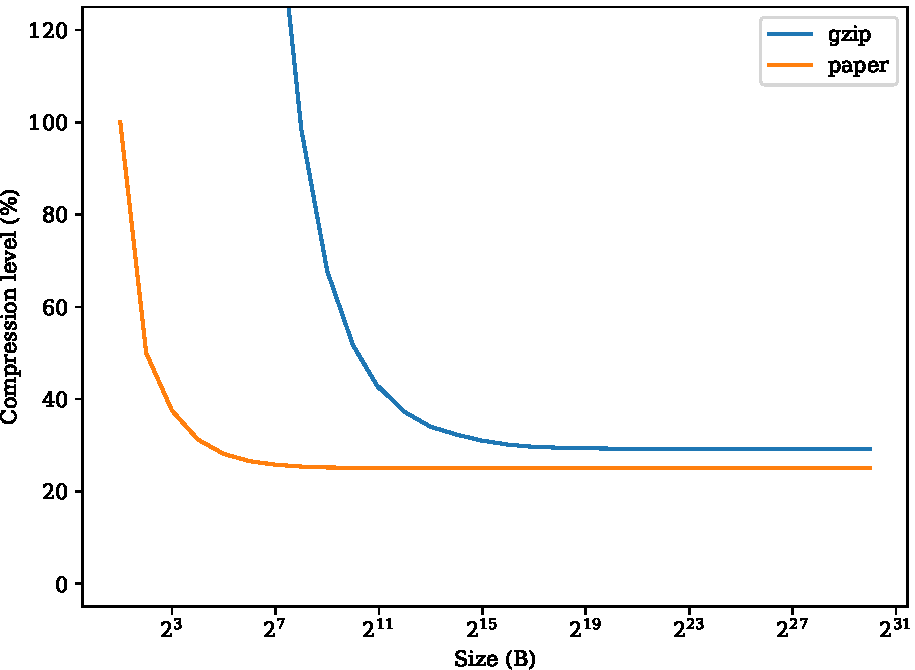
\includegraphics[width=0.95\linewidth]{../plots/compression.pdf}
    \caption{Percentage of compression for each size}
    \label{fig:compression}
\end{figure}

\begin{figure}[htbp]
    \centering
    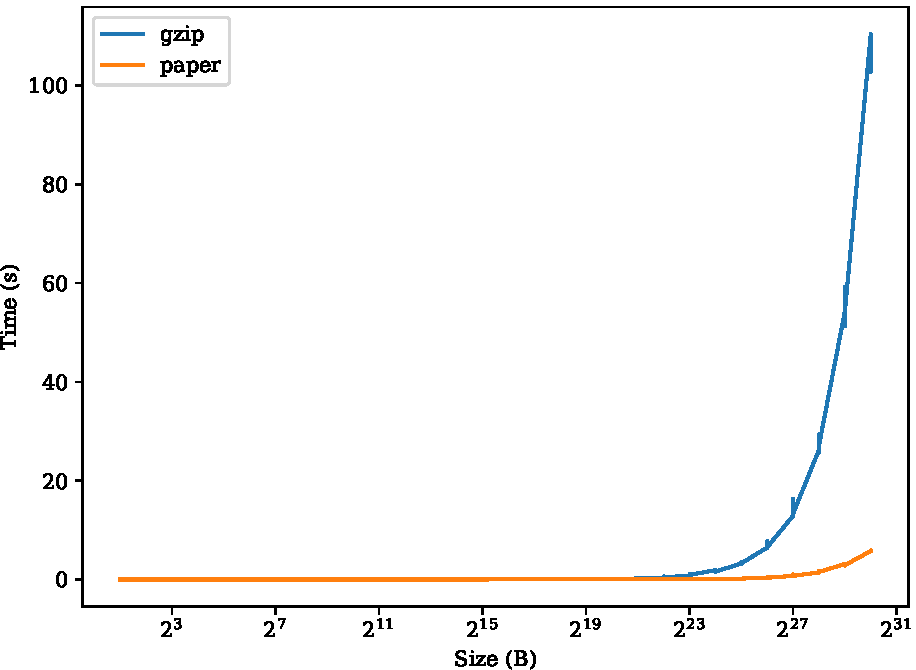
\includegraphics[width=0.95\linewidth]{../plots/time.pdf}
    \caption{Time to compress for each size}
    \label{fig:time}
\end{figure}


\section{Conclusions}
% Your personal conclusions (10\%)

\bibliographystyle{unsrt}
\bibliography{cites}


\end{document}